\documentclass{article}
\usepackage{fontspec}
\usepackage{xeCJK}
\setCJKmainfont{SimSun}

%\usepackage{fontspec}
\usepackage{float}
\usepackage{graphicx}
\usepackage{framed}
\usepackage[inline]{enumitem}
\usepackage{footnote}

\usepackage{caption}
\captionsetup{margin=10pt,font=small,labelfont=bf}
\usepackage{subcaption}

\usepackage[ linktocpage=true]{hyperref}
\hypersetup{
	colorlinks=true,
	breaklinks=true,
	pdfinfo={
		Title={Technical Analysis and Backtesting 
			From Scratch -- A Demonstration},
		Subject={Technical Analysis},
		Author={Kong Shuai},
		Recipients={}
	}
}

\usepackage[numbered]{bookmark}


\begin{document}

\title{技术分析的Python实现\\[2ex]——示例}
\author{孔帅\\
kongshuai89@gmail.com}
\date{May 5, 2013}

\maketitle

\begin{framed}
	\begin{large}注意\end{large}:
	本文档旨在演示已掌握的IT技能在工作中可能提供的帮助。
	文中结论不应视为有现实指导意义\footnotemark。

	\bigskip
	
	请勿公开传播此文档。保留所有权利。
\end{framed}

\footnotetext{主要原因包括:
			\emph{a}) 价格未对股息、分股等进行调整;
			\emph{b}) 价格数据来源被认为并不总是准确的;
			\emph{c}) 没有经过系统的测试以及
			\emph{d}) 没有可信的理论参考。
			}


\section{概览}
项目任务是:支持基于技术分析的交易策略定义,支持基于历史数据的策略评估。
该项目包含三个组成部分:
\begin{itemize}[itemsep=0pt]
\item 数据源,提供交易数据
\item 支持定于与检验的分析框架
\item 交易数据分析
\end{itemize}

\section{数据源}
数据源的任务是提供基础数据,例如成交价量、板块、交易所等信息。
考虑到数据量可能会比较大,数据库选用PostgreSQL。
使用Python脚本下载和更新数据。

\section{分析框架}
考虑到Python的易用性和扩展性,并没有单独定义另外的语言。
这里只是用Python完成了技术分析的框架部分,
自定义的策略与基本的技术分析一样,直接用Python定义。
考虑到执行效率,项目使用了在科学编程中广泛使用的
NumPy\footnote{NumPy is the fundamental package 
for scientific computing with Python.}和
matplotlib\footnote{matplotlib is a Python 2D plotting library 
which produces publication quality figures in a variety of hardcopy 
formats and interactive environments across platforms.}包
完成计算和绘图任务。考虑到大部分程序都能绘制漂亮的分析图,
因此在该项目中只是作为补充,如图~\ref{fig:macd-plot}所示。

\begin{figure}[H]
\centering
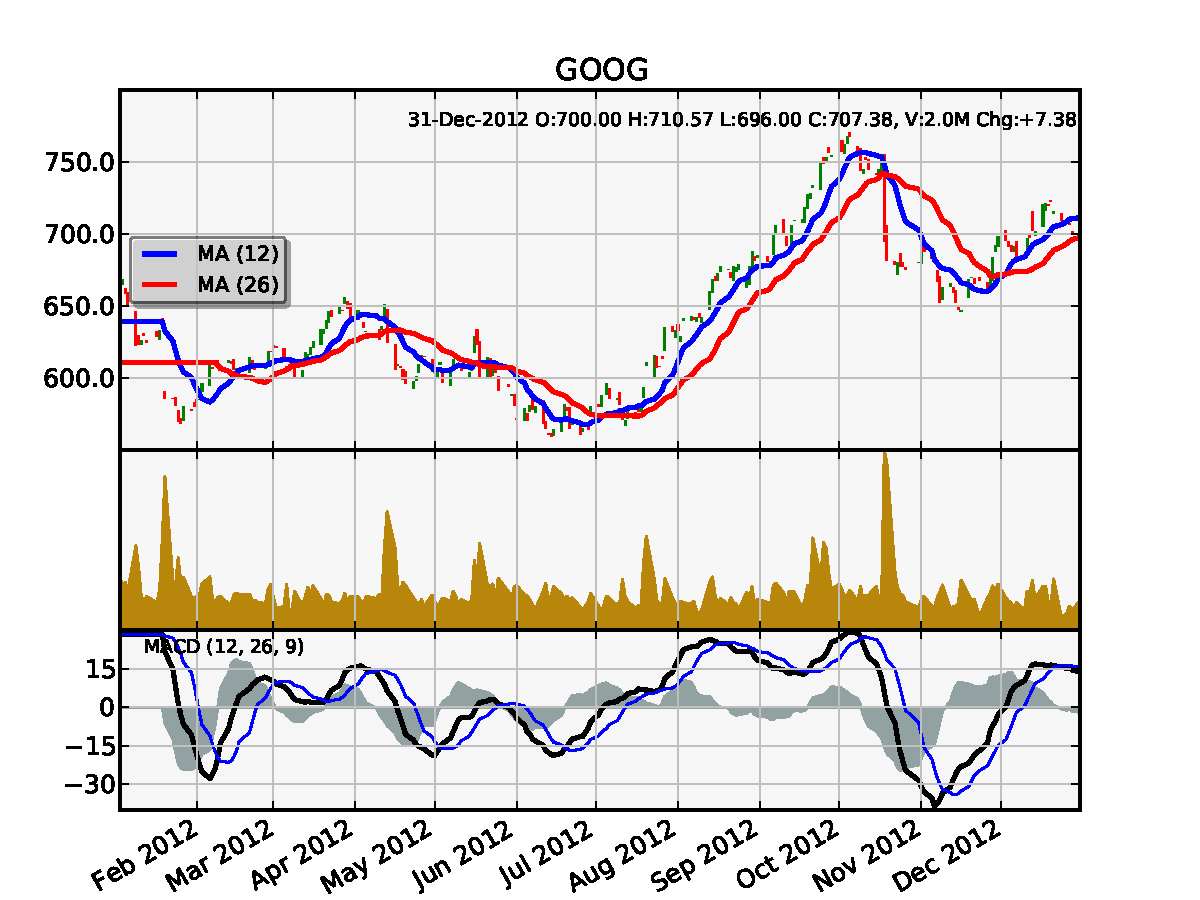
\includegraphics[width=\textwidth]{image/macd-plot.pdf}
\caption{A MACD Figure by Python with Matplotlib\label{fig:macd-plot}}
\end{figure}

\section{数据分析}
使用Python同样能完成数据的分析工作,但基于自定义策略的输出可能是
灵活的,因此分析工作常常也是探索性的,更合适的是使用一种
专门的统计分析工具,本项目使用的是R。

\subsection{演示——MACD的参数}
MACD需要选择三个参数。随着信息化的深入,有理由相信人们对交易数据变化
的反应更加迅速,经典的MACD参数可能已不合适。


在该项目的框架下,容易检验参数选择对收益的影响。作为示意,
以下演示的是对30支DJIA成分股检验仅使用快慢移动平均线交叉的买卖
信号的结果。

\begin{figure}[H]
\begin{subfigure}[b]{.5\textwidth}
\centering
\includegraphics[width=\textwidth, height=!]{image/revenue-nfast2.pdf}
\caption{Revenue of Each $\mathrm{n_{fast}}$}
\label{fig:revenue-by-par:nfast}
\end{subfigure}
\begin{subfigure}[b]{.5\textwidth}
\centering
\includegraphics[width=\textwidth, height=!]{image/revenue-nslow2.pdf}
\caption{Revenue of Each $\mathrm{n_{slow}}$}
\label{fig:revenue-by-par:nslow}
\end{subfigure}
\caption{Revenue Categorized by Parameter Value}
\label{fig:revenue-by-par}
\end{figure}


% latex table generated in R 2.15.2 by xtable 1.7-0 package
% Tue Feb 12 20:20:19 2013
\begin{table}[H]
\caption{Revenue Summary on $\mathrm{n_{fast}}$}
\label{tab:revenue-by-nfast}
\begin{center}
\begin{tabular}{rrrrrrr}
  \hline
 & Min. & 1st Qu. & Median & Mean & 3rd Qu. & Max. \\ 
  \hline
5 & 508.40 & 907.70 & 989.60 & 997.00 & 1062.00 & 1740.00 \\ 
  6 & 501.60 & 924.60 & 1005.00 & 1012.00 & 1081.00 & 1733.00 \\ 
  7 & 505.60 & 939.50 & 1018.00 & 1026.00 & 1097.00 & 1748.00 \\ 
  8 & 503.80 & 953.60 & 1037.00 & 1046.00 & 1117.00 & 1859.00 \\ 
  9 & 491.50 & 960.80 & 1049.00 & 1052.00 & 1125.00 & 1911.00 \\ 
  10 & 473.10 & 958.10 & 1049.00 & 1047.00 & 1128.00 & 1884.00 \\ 
  11 & 486.70 & 953.10 & 1046.00 & 1035.00 & 1122.00 & 1951.00 \\ 
  12 & 479.40 & 938.30 & 1032.00 & 1019.00 & 1114.00 & 1746.00 \\ 
  13 & 461.00 & 943.20 & 1029.00 & 1006.00 & 1105.00 & 1512.00 \\ 
  14 & 463.60 & 941.80 & 1016.00 & 992.20 & 1088.00 & 1488.00 \\ 
  15 & 466.00 & 935.40 & 1005.00 & 982.10 & 1075.00 & 1489.00 \\ 
   \hline
\end{tabular}

\end{center}
\end{table}

\section{总结}

这个高度简化示例的结论不具有现实意义,但演示了Python的一个应用。
在信息技术的帮助下,很多想法得以实现,
有规律的重复工作的效率将得以极大提高。

\end{document}